\documentclass[tikz,border=12pt]{standalone}
\usepackage[T1]{fontenc}
\usepackage{mathpazo}
\usepackage{amsmath,amssymb}
\usetikzlibrary{arrows.meta, positioning, calc, fit, patterns, decorations.pathreplacing}

\definecolor{stblue}{HTML}{7B97AD}
\definecolor{rwgold}{HTML}{B8995E}
\definecolor{sage}{HTML}{7A9A7E}
\definecolor{dkbrown}{HTML}{3D3530}
\definecolor{wmgray}{HTML}{7B7067}
\definecolor{cream}{HTML}{F9F6F0}
\definecolor{border}{HTML}{D4C9B8}
\definecolor{terracotta}{HTML}{C47A6A}
\definecolor{lavender}{HTML}{907EA0}

\begin{document}
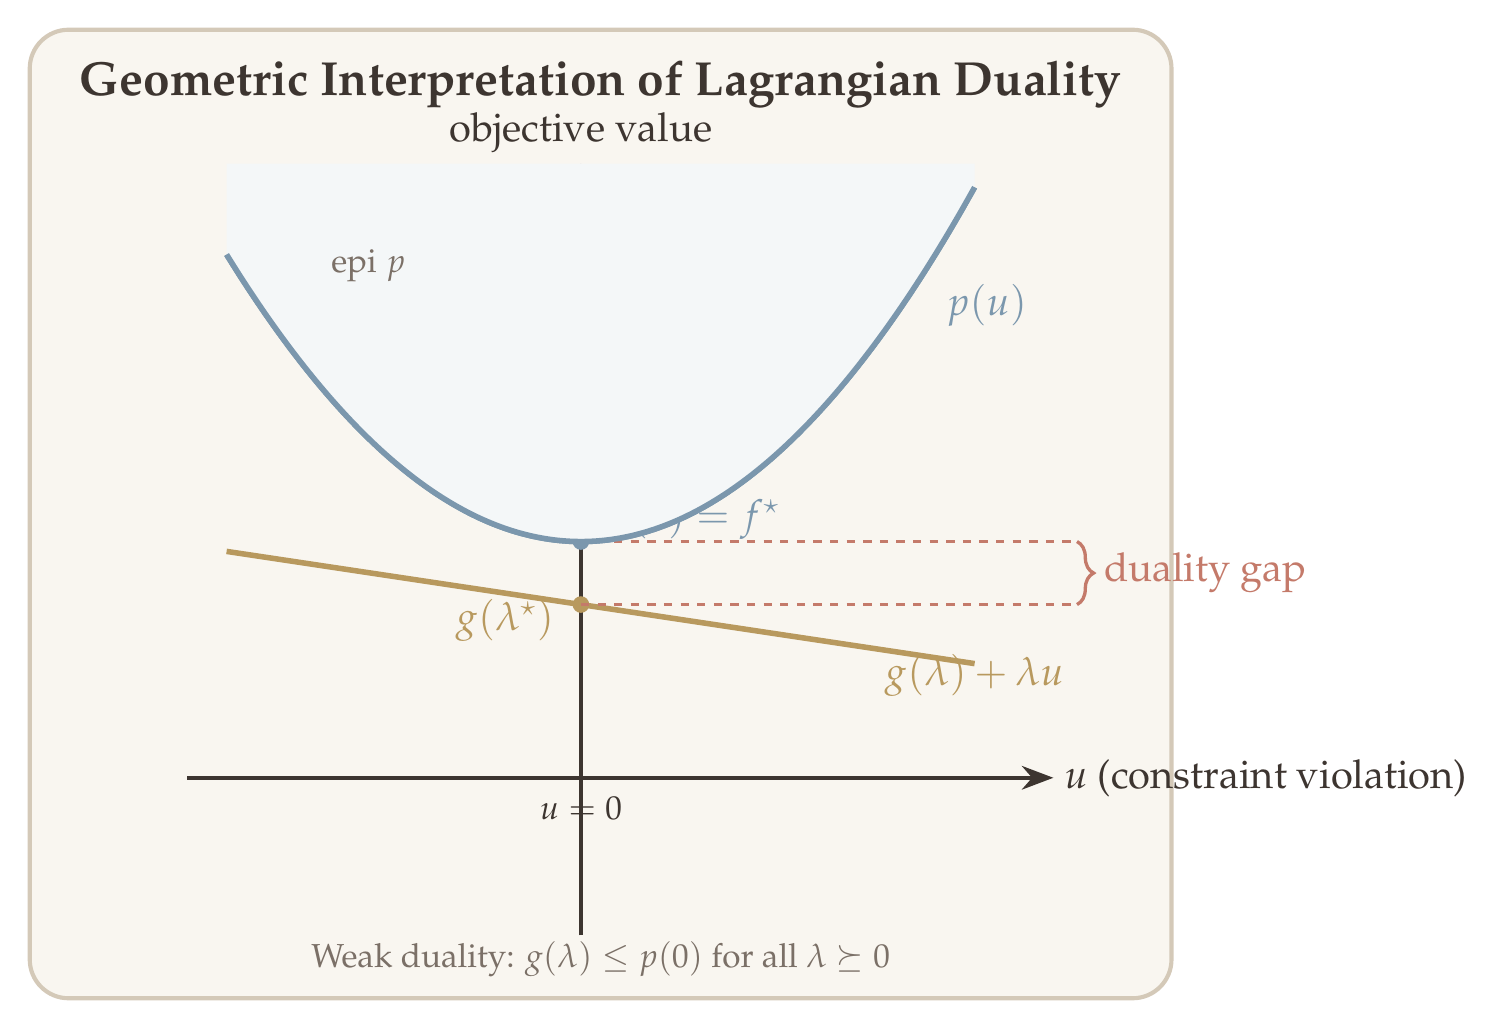
\begin{tikzpicture}[>={Stealth[length=4mm, width=3mm]}, line width=1.5pt]

% Background
\fill[cream, rounded corners=14pt] (-1.5,-2.8) rectangle (13,9.5);
\draw[border, line width=1.5pt, rounded corners=14pt] (-1.5,-2.8) rectangle (13,9.5);

% Title
\node[font=\LARGE\bfseries, text=dkbrown] at (5.75,8.8) {Geometric Interpretation of Lagrangian Duality};

% Axes
\draw[->, dkbrown, line width=1.5pt] (0.5,0) -- (11.5,0) node[right, font=\Large, text=dkbrown] {$u$ (constraint violation)};
\draw[->, dkbrown, line width=1.5pt] (5.5,-2) -- (5.5,7.8) node[above, font=\Large, text=dkbrown] {objective value};

% u=0 dashed line
\draw[dkbrown, dashed, line width=0.8pt] (5.5,-1.6) -- (5.5,7.5);
\node[font=\large, text=dkbrown, below] at (5.5,-0.1) {$u=0$};

% Perturbation function p(u) as a convex curve
\draw[stblue, line width=2pt, smooth, samples=60, domain=1:10.5]
  plot (\x, {0.18*(\x-5.5)*(\x-5.5) + 3.0});
\node[font=\Large, text=stblue, right] at (10,6.0) {$p(u)$};

% p(0) point
\fill[stblue] (5.5,3.0) circle (3pt);
\node[font=\Large, text=stblue, right] at (5.7,3.3) {$p(0) = f^\star$};

% Supporting hyperplane (dual function): g(lambda) + lambda*u at optimal lambda
\draw[rwgold, line width=2pt, domain=1:10.5]
  plot (\x, {-0.15*(\x-5.5) + 2.2});
\node[font=\Large, text=rwgold] at (10.5,1.3) {$g(\lambda) + \lambda u$};

% Dual value at u=0
\fill[rwgold] (5.5,2.2) circle (3pt);
\node[font=\Large, text=rwgold, left] at (5.3,2.0) {$g(\lambda^\star)$};

% Duality gap brace
\draw[decorate, decoration={brace, amplitude=6pt, mirror}, terracotta, line width=1.2pt]
  (11.8,2.2) -- (11.8,3.0);
\node[font=\Large, text=terracotta, right] at (12.0,2.6) {duality gap};

% Duality gap arrows
\draw[terracotta, line width=1pt, dashed] (5.5,2.2) -- (11.8,2.2);
\draw[terracotta, line width=1pt, dashed] (5.5,3.0) -- (11.8,3.0);

% Epigraph shading
\fill[stblue!8, smooth, samples=60, domain=1:10.5]
  plot (\x, {0.18*(\x-5.5)*(\x-5.5) + 3.0}) -- (10.5,7.8) -- (1,7.8) -- cycle;
\node[font=\large, text=wmgray] at (2.8,6.5) {$\mathrm{epi}\; p$};

% Redraw curve on top
\draw[stblue, line width=2pt, smooth, samples=60, domain=1:10.5]
  plot (\x, {0.18*(\x-5.5)*(\x-5.5) + 3.0});

% Annotation
\node[font=\large, text=wmgray, align=center] at (5.75,-2.3)
  {Weak duality: $g(\lambda) \le p(0)$ for all $\lambda \succeq 0$};

\end{tikzpicture}
\end{document}
